\documentclass[UTF8]{ctexart}
\title{基于 Radon 变换及其反投影逆过程的 CT 影像重建方案与单目标投影参数标定优化}
\usepackage{amsmath}
\usepackage{amssymb}
\usepackage{url}
\usepackage{geometry}
\usepackage{appendix}
\usepackage{booktabs}
\usepackage{cases}
\usepackage{graphicx}
\usepackage{subfigure}
\usepackage{listings}
\usepackage{xcolor}
\usepackage{fancyhdr}

\pagestyle{fancy}
\lhead{}
\rhead{}
\chead{}
\lfoot{}
\cfoot{\thepage}
\rfoot{}
\renewcommand{\headrulewidth}{0pt}
\renewcommand{\footrulewidth}{0pt}

\linespread{1.5}
\geometry{left=2.5cm,right=2.5cm,top=2.5cm,bottom=2.5cm}
\bibliographystyle{gbt7714-2005}

\ctexset{
  section = {
      name = \S
  }
}

\begin{document} 
\date{}
\maketitle 

\begin{abstract}

CT(Computed Tomography)可以在不破坏样品的情况下,利用样品对射线能量的吸收特性对生物组织和工程材料的样品进行断层成像,由此获取样品内部的结构信息。在该问题给定条件下,平行入射的X射线垂直于探测器平面,整个发射-接收系统绕某固定的旋转中心逆时针旋转180次。对每一个X射线方向,在具有512个等距单元的探测器上测量经位置固定不动的二维待检测介质吸收衰减后的射线能量,并经过增益等处理后得到180组接收信息。

对于问题一,在CT系统标定参数未知的情况下,我们需要通过给定的投影数据来确定CT系统旋转中心在正方形托盘中的位置、探测器单元之间的距离以及该CT系统使用的X射线的180个方向。由Lambert-Beer定律对给定数据进行处理得到实际透射厚度,然后我们先利用小圆与射线的关系得到各探测单元间的距离,再采用解析几何方法,将弦长公式与平行线间距离公式联立求得180个方向分别对应的X射线的直线斜率,进而求出其方向,同时也得到了每个方向上各射线的具体方程,接着又采用三角形内切圆法及相对运动法求解转轴的坐标。

对于问题二、三,我们需要问题一中求得的的标定参数以及系统得到的某未知介质的接收信息来还原该断面未知介质在正方形托盘中的位置、几何形状和吸收率等信息,所以这是第一问求解的逆过程。我们知道CT系统的数据处理与Radan变换及逆变换密切相关,于是在这里我们采用Radon逆变换来对未知介质进行还原;另外,附件提供的是离散的投影数据点,而Radon逆变换本身的连续形式在该情况下不适用,所以这里我们将离散数据连续化处理之后,对探测器所在角度、探测器与旋转中心距离的离散数据进行插值,获得近似的连续投影函数,并进行二重积分数值求解,进而求得未知介质的相关信息,再在相同的模型下求得10个位置的透射率的信息。

对于问题四,我们通过两种方案对参数的精度和稳定性进行分析及改善。在问题二、三的求解中我们用到了二重积分数值求解的方法求解了未知介质的吸收率函数,再通过余项对间距、平均旋转角的标定参数求运用梯度下降优化法,来得到较优的标定参数;也可用遗传算法确定优质标定方案,为了简化计算量、获得直观效果,以一个在正方形托盘范围内的圆作为模板,控制探测器间距一定,半径、圆心坐标、扫描角度均为可变量,使用 MATLAB 提供的 Radon 变换方案进行适合度函数的计算与评估。


\begin{flushleft}
\textbf{关键词:} Radon 变换; 反投影重建算法; 多元目标函数优化
\end{flushleft}
\end{abstract}

\clearpage

\section{题目重述}
\subsection{引言}
\subsubsection{问题背景}

随着当今科技的发展,人们正尝试使用计算机实现越来越多的功能,从而为人们的生活提供便利。当然,计算机在医疗领域中也得到了广泛的应用,例如,计算机可以通过断层成像进行一些影像诊断学的检查,这一技术又称“电脑断层扫描(Computed Tomography)”,简称为CT。CT将计算机与X射线相结合,将X射线扫描结果通过信号转换转为数字形式,导入计算机中进行数据存储及处理,最后在显示器上直观显示图像,从而应用于医疗领域。

CT可以在不破坏样品的情况下,通过不同角度对物体进行扫描,使探测器接收到经过物体后衰减的X射线量,通过计算机处理数据对生物组织和工程材料的样品进行断层成像,由此获取样品内部的结构信息,以便进行后续的判断或研究。

CT系统主要包含扫描系统、计算机处理系统、图像显示系统三部分。其中,扫描系统由X射线发射器、探测器和扫描架组成。

\subsubsection{问题产生}
一种典型的二维CT系统如图1所示,平行入射的X射线垂直于探测器平面,每个探测器单元看成一个接收点,且等距排列。X射线的发射器和探测器相对位置固定不变,整个发射-接收系统绕某固定的旋转中心逆时针旋转180次。对每一个X射线方向,在具有512个等距单元的探测器上测量经位置固定不动的二维待检测介质吸收衰减后的射线能量,并经过增益等处理后得到180组接收信息。

CT系统安装时往往存在误差,从而影响成像质量,因此需要对安装好的CT系统进行参数标定,即借助于已知结构的样品(称为模板)标定CT系统的参数,并据此对未知结构的样品进行成像。

\subsection{需解决的具体问题}
\begin{enumerate}
\item 在正方形托盘上放置两个均匀固体介质组成的标定模板,模板的几何信息如图2所示,相应的数据文件见附件1,其中每一点的数值反映了该点的吸收强度,这里称为“吸收率”。对应于该模板的接收信息见附件2。请根据这一模板及其接收信息,确定CT系统旋转中心在正方形托盘中的位置、探测器单元之间的距离以及该CT系统使用的X射线的180个方向。
\item 附件3是利用上述CT系统得到的某未知介质的接收信息。利用问题1中得到的标定参数,确定该未知介质在正方形托盘中的位置、几何形状和吸收率等信息。另外,请具体给出图3所给的10个位置处的吸收率,相应的数据文件见附件4。
\item 附件5是利用上述CT系统得到的另一个未知介质的接收信息。利用问题1中得到的标定参数,给出该未知介质的相关信息。另外,请具体给出图3所给的10个位置处的吸收率。
\item 分析问题1中参数标定的精度和稳定性。在此基础上自行设计新模板、建立对应的标定模型,以改进标定精度和稳定性,并说明理由。
\end{enumerate}

\begin{center}
\begin{figure}[htbp]
\centering
\begin{minipage}[t]{0.3\textwidth}
  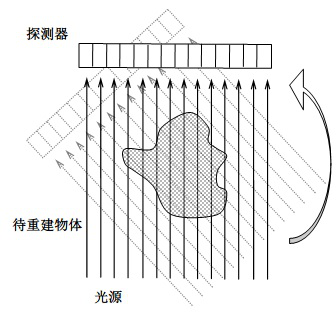
\includegraphics[width=2in]{../figure/problem_1.png}
  \caption{CT系统示意图}
  \label{fig:problem_1}
\end{minipage}
\begin{minipage}[t]{0.3\textwidth}
  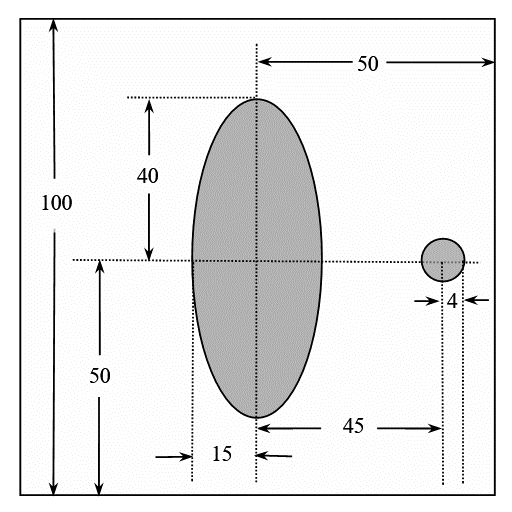
\includegraphics[width=2in]{../figure/problem_2.png}
  \caption{模板示意图(单位:mm)}
  \label{fig:problem_2}
\end{minipage}
\begin{minipage}[t]{0.3\textwidth}
  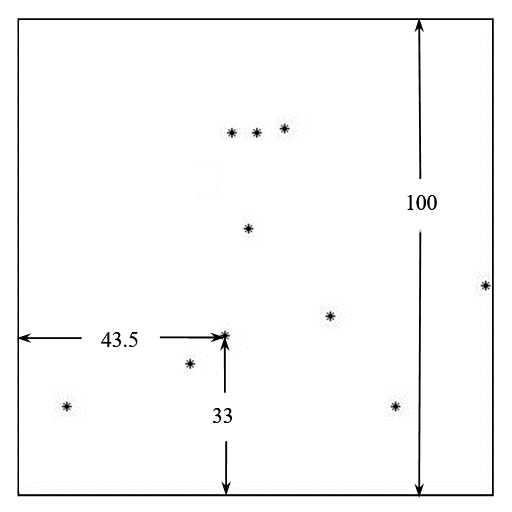
\includegraphics[width=2in]{../figure/problem_3.png}
  \caption{10个位置示意图}
  \label{fig:problem_3}
\end{minipage}
\end{figure}
\end{center}



\section{问题分析}
\subsection{整体问题分析}

本题为CT系统参数标定及成像问题,是一个通过X射线经过待测介质后的衰减量来进行断层成像,从而获取样品内部结构信息的过程。由此,我们联想到了 Radon 变换过程。 Radon 变换是一个对二维平面做线积分(即在某个方向上的积分)的过程,经常被应用于CT成像中,且 Radon 逆变换可以实现对样本的还原,与本题原理相符。

\subsection{具体问题分析}
\subsubsection{对于问题一的分析}

问题一需要参照附件一中模板几何图形的信息和附件二中该模板的接收信息,利用椭圆和圆的性质,结合吸收强度(也称为“吸收率”)的定义,采用 Radon 变换的方法,建立基础解析几何的模型,运用基本的数学运算进行求解,以求得的相关CT系统参数。

\subsubsection{对于问题二、三的分析}

问题二、三类似,均为问题一的逆过程,需采用 Radon 逆变换,即利用问题一解出的系统参数,通过对某介质的接受信息,反推出介质的位置、几何形状和吸收率等信息,并针对的十个具体位置计算其吸收率。据观察数据,两问题的区别在于其余介质对系统的干扰大小。

\subsubsection{对于问题四的分析}

问题四为优化问题,通过问题二、三对问题一所求参数的应用,确定该组参数的精度和稳定性,并对其进行多目标参数优化,加以改进。



\section{模型假设}
\begin{itemize} 
\item  忽略X射线因散射而引起的衰减量;
\item  忽略空气等其他介质对X射线的衰减影响;
\item  假设正方形托盘外无任何介质干扰;
\item  假设将每个探测器单元看成一个接收点,且等距排列。
\end{itemize} 



\section{符号说明}

\begin{table}[htbp]
\centering
\begin{center} 
\begin{tabular}{cc} 
\toprule
\makebox[0.3\textwidth][c]{符号}  &  \makebox[0.4\textwidth][c]{符号说明} \\ \midrule 
$r_0$  &  圆形样本的名义半径  \\  
$r_{real}$  &  圆形样本的实际半径( $mm$ )  \\  
$d$  &  探测器单元之间的名义距离  \\  
$d_{real}$  &  探测器单元之间的实际距离( $mm$ )  \\
$\mu$  &  线吸收系数  \\  
$\iota$  &  X射线衰减程度  \\ 
$l$  &  X射线穿过样本的距离( $mm$ )  \\
$r'$  &  相对旋转半径  \\ 
\bottomrule 
\end{tabular} 
\end{center}
\end{table}



\section{模型建立与求解}
\subsection{问题一}
\subsubsection{问题一的分析}

对于探测器单元之间的距离,用椭圆或圆来求解均可,但为了计算的简洁性,我们在此选取均匀的圆形样本进行计算,利用其中心对称性简化问题;
对于CT系统旋转中心在正方形托盘中的位置,需要利用椭圆求解,在发射-接收系统旋转过程中,可任意选取探测器其中一个单元接收的三个不同角度的射线所在直线,那么这三条直线围成三角形的内切圆的圆心即为旋转中心的位置;
而对于该CT系统使用的X射线的180个方向,由于题中未说明系统是均匀转动的,所以我们将其看做转动不均匀来求解,即分别在180个角度上求解。

在针对各个参数具体建模求解前,我们要对已知条件进行充分的理解。首先,我们用附件二中的所有数据通过 Radon 变换在 Matlab 中生成图像,如图 \ref{fig:matlab} 所示。

\begin{figure}[htbp]
  \centering
  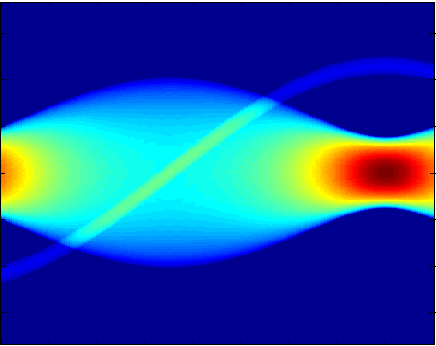
\includegraphics[width=5in]{../figure/matlab.png}
  \caption{经Radon变换处理后X射线检测数据图像}
  \label{fig:matlab}
\end{figure}

由图 \ref{fig:matlab} 观察可知,正弦型窄线描述圆形样本的衰减强度、中间段非对称波浪形宽线描述椭圆样本的衰减强度。由于圆形样本先逐渐靠近探测器中心而后又逐渐远离,故探测器初始位置应大概平行于圆形、椭圆样本中心的连线;由于本题中我们采用的方法为 Radon 线积分,无确切的方向性,故我们假设探测器初始时位于两样本上方且从左至右分别为1至512号探测单元;在图 \ref{fig:matlab} 中还可看出,两样本分别产生的图像先逐渐接近至重合,再由重合逐渐远离,且重合前两图像间距逐渐减小,而重合后两图像间距先大后小,故探测器的初始位置应在样本上方偏左的位置上,而终止位置应在样本下方偏右的位置上,具体如图 \ref{fig:position} 所示(图中为了方便理解,仅画出了探测器起始、终止的大致位置,角度还并未确定)。

\begin{figure}[htbp]
  \centering
  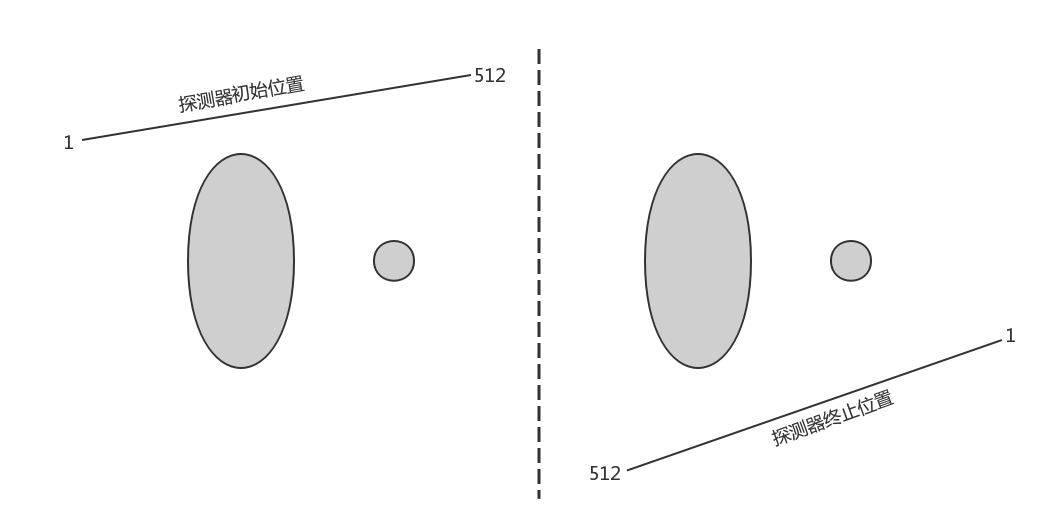
\includegraphics[width=6in]{../figure/position.png}
  \caption{探测器初始、终止位置示意图}
  \label{fig:position}
\end{figure}

在此基础上,我们开始对各个参数分别展开具体的建模求解过程。

\subsubsection{对探测器单元间距的模型建立及求解}

由于我们想利用均匀圆形样本的中心对称性在此题中求解,故我们应考虑射线只通过圆形样本的衰减量,所以为了避免椭圆样本的干扰,我们在此截取了附录二中 EO 列 45-73 行中的部分数据进行对比分析,如表 \ref{danyuan} 所示,以垂直当前射线的方向从圆形样本两侧分别向圆心计数,相互对应的X射线衰减量并非对称相等,而这与均匀圆形样本的中心对称性质相违背,故可说明没有一条射线精准穿过该圆形样本的圆心。

\begin{table}[htbp]
\centering
\caption{圆形样本某一角度的射线衰减量}
\label{danyuan}
\begin{tabular}{c|ccccccccc}
\hline
从左侧计数 & 3.0515 & 5.9598 & 7.7332 & 9.0643 & 10.1289 & 11.0046 & 11.7339 & 12.3427 & ... \\
\hline
从右侧计数 & 3.9356 & 6.4231 & 8.0683 & 9.3281 & 10.3444 & 11.1836 & 11.8834 & 12.4672 & ... \\
\hline
\end{tabular}
\end{table}

附录二中的数据表示的是X射线通过物体后的衰减量,由对大量数据的分析观察可得,X射线衰减程度与穿透物体的距离成正比,并设其比例系数为 $\mu$ 。我们知道,衰减至少应被视为物质对入射线的散射和吸收的结果,系数 $\mu$ 应该是这两部分作用之和,但由于因散射而引起的衰减远小于因吸收而引起的衰减,故通常直接称 $\mu$ 为线吸收系数,而忽略散射的部分。在此,我们对X射线衰减量进行等效,作为圆形样本在此方向上的名义弦长,从而求出圆形样本的名义半径 $r_0$ 和探测器单元之间的名义距离 $d$ 。显然,圆形样本的名义半径与实际半径、探测器单元之间的名义距离与实际距离仍成正比,比例系数均为 $\mu$ 。为了方便列式求解,我们模拟出一个简单的样本模型,如图 \ref{fig:circle} 所示。

\begin{figure}[htbp]
  \centering
  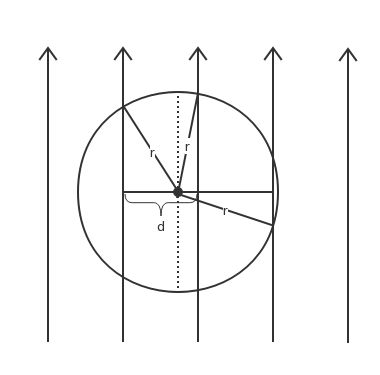
\includegraphics[width=2.5in]{../figure/circle.png}
  \caption{简单模拟圆形样本模型}
  \label{fig:circle}
\end{figure}

在穿过圆形样本的众多射线中,可在表 \ref{danyuan} 中提供的数据中选取任意三条射线的衰减量,利用名义弦长的 1/2 、 $r_0$ 与 $d$ 进行勾股定理的运算,建立关于 
$r_0$ 和 $d$ 的二元方程组,进行求解。具体列式如式(1)所示:

\begin{equation}
  \begin{cases}
    \sqrt{r_0^2-(3.0515/2)^2}+\sqrt{r_0^2-(12.4672/2)^2}=21d \\
    \sqrt{r_0^2-(3.0515/2)^2}+\sqrt{r_0^2-(3.9356/2)^2}=28d  \\
  \end{cases}
\end{equation}

解方程组得:
$$r_0=7.0898,d=0.4905$$

由图 \ref{fig:problem_2} 中已知数据可得,圆形样本的实际半径 $r_{real}$ 为 4 ,由此可计算样本的吸收率 $\mu$ ,即
$$ \mu = \frac{r}{r_{real}} = \frac{7.0898}{4} = 1.7725 $$

由此可得,探测器单元之间的实际距离应为
$$ d_{real} = \frac{d}{\mu} = \frac{0.4905}{1.7725} = 0.2767mm $$
则此 $d_{real}$ 即为本题所求。

此外,还可知X射线衰减程度 $\iota$ 与穿透物体的距离 $l$ 之间的关系为
$$ \iota = 1.7725*l $$

\subsubsection{对CT系统旋转中心的模型建立及求解}

\textbf{解法一:用三角形内切圆法求旋转中心坐标}

为了求得CT系统旋转中心在正方形托盘中的位置,我们以椭圆中心为原点、横向为 $x$ 轴、纵向为 $y$ 轴建立直角坐标系,并针对给定模板建立了基础解析几何的模型,如图 \ref{fig:oval} 所示。

\begin{figure}[htbp]
  \centering
  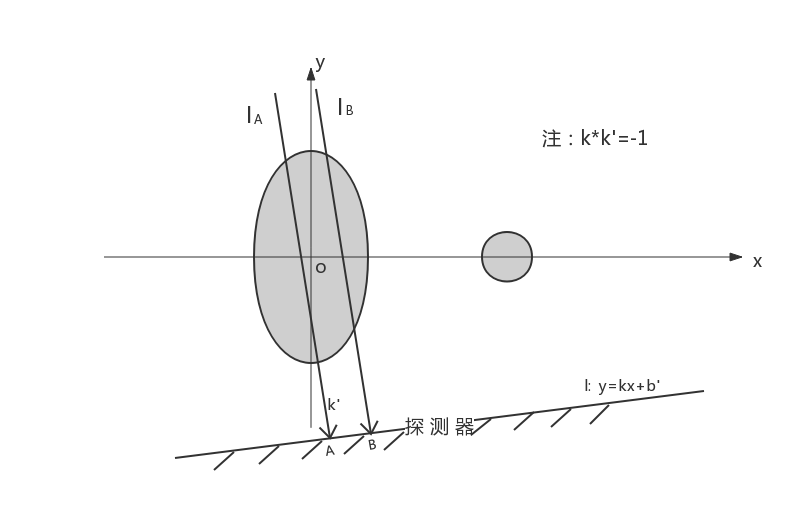
\includegraphics[width=5in]{../figure/oval.png}
  \caption{解析几何模型}
  \label{fig:oval}
\end{figure}

其中,椭圆方程为

\begin{equation}
\label{equ:oval}
 \frac{x^2}{a^2}+ \frac{y^2}{b^2}=1 
\end{equation}

两条射线的解析方程为

\begin{equation}
\label{equ:line}
  \begin{cases}
    l_A: y=k'x+b_1' \\
    l_B: y=k'x+b_2'  \\
  \end{cases}
\end{equation}

将式(\ref{equ:oval})与(\ref{equ:line})联立,得到

\begin{equation}
\label{equ:x}
  \begin{cases}
    x_{1,2}=\dfrac{-\dfrac{2k'a^2}{b^2}\pm\sqrt{\dfrac{4k'^2a^4b_1'^2}{b^4}-4a^2(1+\dfrac{a^2}{b^2}k'^2)(\dfrac{b_1'^2}{b^2}-1)}}{2(1+\dfrac{a^2}{b^2}k'^2)}  \\
    x_{3,4}=\dfrac{-\dfrac{2k'a^2}{b^2}\pm\sqrt{\dfrac{4k'^2a^4b_2'^2}{b^4}-4a^2(1+\dfrac{a^2}{b^2}k'^2)(\dfrac{b_2'^2}{b^2}-1)}}{2(1+\dfrac{a^2}{b^2}k'^2)}  \\
  \end{cases}
\end{equation}
其中, $x_{1,2}$ 为 $l_A$ 与椭圆的两个交点、 $x_{3,4}$ 为 $l_B$ 与椭圆的两个交点,而且上式应满足 $\Delta=\dfrac{4k'^2a^4}{b^4}-4a^2(1+\dfrac{a^2}{b^2}k'^2)(\dfrac{b_1'^2}{b^2}-1)\geq0$ 。

将式(\ref{equ:x})带入通用椭圆弦长公式 $l=|\Delta x|\sqrt{1+k^2}$ 中,可以得到
\begin{equation}
\label{equ:xian}
  \begin{cases}
    l_1=\dfrac{\sqrt{1+k'^2}}{(1+\dfrac{a^2}{b^2}k'^2)}\sqrt{\dfrac{4k'^2a^4b_1'^2}{b^4}-4a^2(1+\dfrac{a^2}{b^2}k'^2)(\dfrac{b_1'^2}{b^2}-1)}  \\
    l_2=\dfrac{\sqrt{1+k'^2}}{(1+\dfrac{a^2}{b^2}k'^2)}\sqrt{\dfrac{4k'^2a^4b_2'^2}{b^4}-4a^2(1+\dfrac{a^2}{b^2}k'^2)(\dfrac{b_2'^2}{b^2}-1)}  \\
    d=\dfrac{|b_1'-b_2'|}{\sqrt{1+k'^2}}  \\
  \end{cases}
\end{equation}

其中, $l_1$ 、 $l_2$ 分别为直线 $l_A$ 、$l_B$ 与椭圆相交所得的弦长,且所有弦长均可在附件二中查找到具体数值,故在此可任意选取512条射线中的任意条射线在任意角度上的衰减量,举例如表 \ref{lineexp} 所示。

\begin{table}[htbp]
\centering
\caption{任意射线任意角度衰减量对应弦长举例}
\label{lineexp}
\begin{tabular}{cccc}
\toprule
  & 角度一对应弦长(A列) & 角度二对应弦长(M列) & 角度三对应弦长(FN列)  \\
\midrule
射线一(第207条) & 55.3699/$\mu$ & 60.5585/$\mu$ & 103.6913/$\mu$  \\
射线二(第209条) & 57.9461/$\mu$ & 61.5168/$\mu$ & 104.8858/$\mu$  \\
\bottomrule
\end{tabular}
\end{table}

我们选取表 \ref{lineexp} 中射线进行计算,将三列数据分别带入式(\ref{equ:xian})中依次计算,并确定出合乎条件的方程组解集,此时我们得到了三组平行射线 $l_A$ 、$l_B$ 的解析式,在此选取 $l_A$ 的三个解析式(表示第207个单元的探测器在三个不同角度接收的射线所在直线),如式(\ref{equ:threeline})所示。

\begin{equation}
\label{equ:threeline}
  \begin{cases}
    y_1=-1.6643x-30.7476  \\
    y_2=-0.9777x-21.9452  \\
    y_3=2.8012x+21.0629  \\
  \end{cases}
\end{equation}

由此三条直线可求得三个交点以及每个角的角度,进而求得三条直线的内切圆圆心(三条直线形成三角形的三个内角分线的交点),此点即为系统的旋转中心。如图 \ref{fig:threeline} 所示,其中红线为 $y_1$ 图像、绿线为 $y_2$ 图像、蓝线为 $y_3$ 图像。

\begin{figure}[htbp]
  \centering
  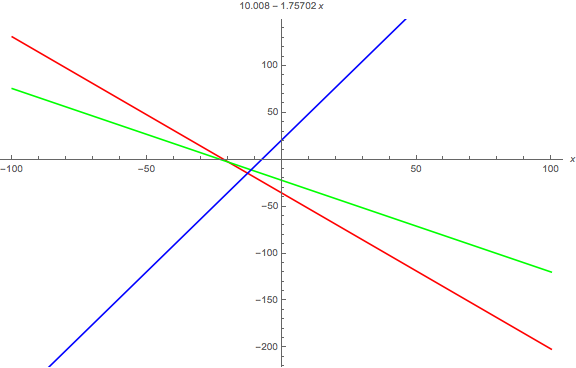
\includegraphics[width=3in]{../figure/threeline.png}
  \caption{三条直线示意图}
  \label{fig:threeline}
\end{figure}

通过编程,我们求得该内切圆圆心坐标为(-6.0874, 4.1505),这一点即为CT系统旋转中心的位置,位于椭圆圆心的左下方且在椭圆内部。

\textbf{解法二:用相对运动求解旋转中心对探测器的相对坐标}

我们还可以转换参考系,假定探测器不动而样本绕探测器顺时针移动。我们在此选取某一个单元接收点 $x_i$ 以及任意三个圆相对于探测器的位置,并保证三个角度下的圆形样本均被 $x_i$ 穿过且圆心均在 $x_i$ 同一侧,如局部图 \ref{fig:detail} 所示。

\begin{figure}[htbp]
  \centering
  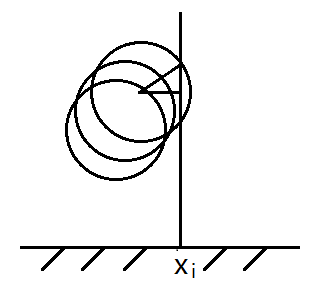
\includegraphics[width=1.5in]{../figure/detail.png}
  \caption{相对坐标系局部细节图}
  \label{fig:detail}
\end{figure}

在图 \ref{fig:detail} 中,弦长、圆半径已知,可由勾股定理求出圆心距 $x_i$ 的距离,则在整体图 \ref{fig:roar} 中, $x_1$ 、 $x_2$ 、 $x_3$ 均可求。 

\begin{figure}[htbp]
  \centering
  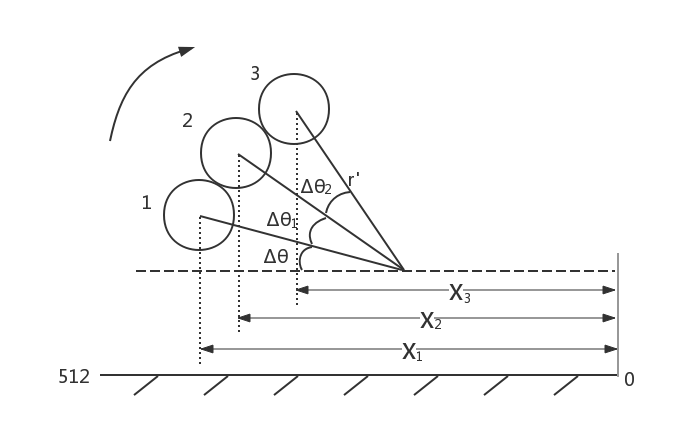
\includegraphics[width=4.5in]{../figure/roar.png}
  \caption{相对坐标系示意图}
  \label{fig:roar}
\end{figure}

然后通过下式求得圆心的旋转半径 $r'$ :

$$
\begin{cases}
  r'\cos\Delta\theta-r'\cos(\Delta\theta+\Delta\theta_1)=x_1-x_2 \\
  r'\cos\Delta\theta-r'\cos(\Delta\theta+\Delta\theta_1+\Delta\theta_2)=x_1-x_3 \\
\end{cases}
$$

由此易求得CT系统的旋转中心。

\subsubsection{对CT系统射线180个方向的模型建立及求解}

对于未知180个方向是否均匀分布的情况,我们暂且视为不均匀,分别针对每个方向计算,此处仍利用椭圆样本进行求解。具体求解方法为:在每个角度上任取两个数据作为椭圆弦长,再带入到椭圆联立得到的弦长方程式(\ref{equ:xian})中,解出当前角度下射线所在直线的方程式,由其斜率即可得到该方向的角度。

为了不受两个样本的累加作用而影响计算、又能使计算做到尽量简洁,我们在此统一在前九十个方向上取附件二中自上至下的第三个和第十个非零数据、在后九十个方向上取自下至上的第三个和第十个非零数据,具体取值情况如图 \ref{fig:angle} 所示,图中红色位置为大致取值区域。

\begin{figure}[htbp]
  \centering
  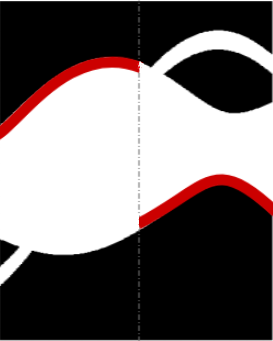
\includegraphics[width=2.5in]{../figure/angle.png}
  \caption{计算角度取值大致区域示意图}
  \label{fig:angle}
\end{figure}

通过编程进行计算,得到180次旋转的平均弧度为 0.0175 ,即平均每次旋转转动 $1.0028^{\circ}$ 角,且X射线照射的初始方向的弧度为 2.0882 ,即与坐标轴的x正半轴成 $119.6539^{\circ}$ 角。由于 Matlab 不能计算出特定某些位置的角度,故在我们改为手动计算,算得具体的180个方向如下(以弧度表示):

前九十个方向:

2.0882 ; 2.1118 ; 2.1215 ; 2.1406 ; 2.1586 ; 2.1755 ; 2.1929 ; 2.2104 ; 2.2278

2.2453 ; 2.2628 ; 2.2802 ; 2.2977 ; 2.3151 ; 2.3326 ; 2.3526 ; 2.3675 ; 2.3849

2.4024 ; 2.4198 ; 2.4373 ; 2.4547 ; 2.4722 ; 2.4896 ; 2.5071 ; 2.5246 ; 2.5420

2.5595 ; 2.5769 ; 2.5944 ; 2.6118 ; 2.6275 ; 2.6467 ; 2.6642 ; 2.6815 ; 2.6990

2.7165 ; 2.7340 ; 2.7514 ; 2.7689 ; 2.7864 ; 2.8038 ; 2.8213 ; 2.8387 ; 2.8562

2.8736 ; 2.8911 ; 2.9085 ; 2.9260 ; 2.9434 ; 2.9608 ; 2.9783 ; 2.9958 ; 3.0133

3.0307 ; 3.0482 ; 3.0656 ; 3.0831 ; 3.1005 ; 3.1180 ; 3.1357 ; 3.1527 ; 3.1703

3.1878 ; 3.2053 ; 3.2227 ; 3.2401 ; 3.2576 ; 3.2750 ; 3.2925 ; 3.3100 ; 3.3274

3.3449 ; 3.3623 ; 3.3798 ; 3.3972 ; 3.4147 ; 3.4321 ; 3.4496 ; 3.4670 ; 3.4845

3.5019 ; 3.5194 ; 3.5369 ; 3.5543 ; 3.5718 ; 3.5892 ; 3.6067 ; 3.6206 ; 3.6416

后九十个方向:

3.6590 ; 3.6765 ; 3.6939 ; 3.7114 ; 3.7288 ; 3.7463 ; 3.7637 ; 3.7812 ; 3.7986

3.8161 ; 3.8336 ; 3.8510 ; 3.8702 ; 3.8859 ; 3.9034 ; 3.9208 ; 3.9383 ; 3.9557

3.9732 ; 3.9906 ; 4.0081 ; 4.0255 ; 4.0430 ; 4.0604 ; 4.0779 ; 4.0954 ; 4.1128

4.1303 ; 4.1477 ; 4.1652 ; 4.1826 ; 4.2001 ; 4.2175 ; 4.2350 ; 4.2524 ; 4.2699

4.2873 ; 4.3048 ; 4.3222 ; 4.3397 ; 4.3571 ; 4.3746 ; 4.3921 ; 4.4095 ; 4.4270

4.4444 ; 4.4619 ; 4.4793 ; 4.4968 ; 4.5142 ; 4.5317 ; 4.5491 ; 4.5666 ; 4.5840

4.6015 ; 4.6190 ; 4.6364 ; 4.6539 ; 4.6713 ; 4.6888 ; 4.7062 ; 4.7237 ; 4.7411

4.7586 ; 4.7760 ; 4.7935 ; 4.8109 ; 4.8284 ; 4.8458 ; 4.8633 ; 4.8807 ; 4.8982

4.9157 ; 4.9331 ; 4.9506 ; 4.9680 ; 4.9855 ; 5.0029 ; 5.0204 ; 5.0378 ; 5.0553

5.0727 ; 5.0902 ; 5.1076 ; 5.1251 ; 5.1425 ; 5.1600 ; 5.1775 ; 5.1949 ; 5.2122



\subsection{问题二}
\subsubsection{问题二的分析}

在此问题中,我们需要问题一中求得的的标定参数以及系统得到的某未知介质的接收信息来还原该断面未知介质在正方形托盘中的位置、几何形状和吸收率等信息,所以这是第一问求解的逆过程。我们知道CT系统的数据处理与 Radan 变换及逆变换密切相关,于是在这里我们采用 Radon 逆变换来对未知介质进行还原;另外,附件提供的是离散的投影数据点,而Radon逆变换需要的是投影函数对转心到射线距离的偏导数,所以这里我们采用 Matlab 中的 iradon 函数对离散数据进行插值的方法获得近似投影函数并进行 Radon 逆变换,进而求得未知介质的相关信息。

\subsubsection{逆 Radon 反投影变换与滤波过程模型的建立及求解}

在本问题中,我们将附件中提供的大量离散点通过插值得到光滑连续的投影函数,再通过 Radon 逆变换的方式求得重建图像函数。首先我们要了解 Radon 变换,示意图如图 \ref{fig:radon} 所示。

\begin{figure}[htbp]
  \centering
  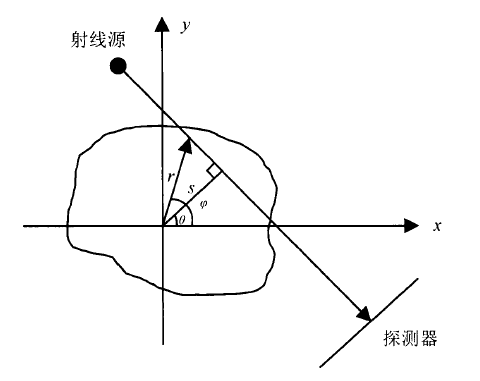
\includegraphics[width=3.5in]{../figure/radon.png}
  \caption{Radon 变换示意图}
  \label{fig:radon}
\end{figure}

依据郭静钰等人\cite{郭静钰2016有限角度}、Anderson 等人\cite{andersen1984simultaneous}的研究成果,我们设实际样本的吸收率分布矩阵中各点组成的离散型函数为原函数 $f(x,y)$ ,对该平面内任意一条射线 $L$ 进行线积分,得到经 Radon 变换后的函数
\begin{equation}
\label{equ:radon}
 p(s,\theta) = \int_L f(x,y) \mathrm{d}l = \int_{-\infty}^{+\infty}\int_{-\infty}^{+\infty}f(x,y)\delta(x\cos\theta+y\sin\theta-s)\mathrm{d}x \mathrm{d}y
\end{equation}

式(\ref{equ:radon})中, $s$ 是原点到射线 $L$ 的距离,$\theta$ 是射线 $L$ 所在直线的法向量与x轴的夹角,具体如图 \ref{fig:radon} 所示。

由式(\ref{equ:radon})可求得逆 Radon 变换的公式为:
$$ f_1(x,y)=\frac{1}{2\pi^2}\int_0^\pi\int_{-\infty}^{+\infty}\frac{1}{r\cos(\varphi-\theta)-s}\frac{\partial p(s,\theta)}{\partial s}\mathrm{d}s\mathrm{d}\theta $$

接下来,我们进行 Radon 逆变换,采用Matlab中的 iradon 函数对投影函数 $p(s,\theta)$ 进行运算,得到的介质图像如图 \ref{fig:answer_2} 所示。

\begin{figure}[htbp]
  \centering
  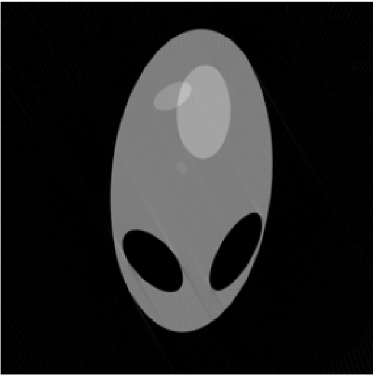
\includegraphics[width=3in]{../figure/answer_2.png}
  \caption{Randon 逆变换还原结果图}
  \label{fig:answer_2}
\end{figure}

解得图 \ref{fig:problem_3} 提供的十个位置处的吸收率如表 \ref{problem_2} 所示。

\begin{table}[htbp]
\centering
\caption{十个位置处的吸收率}
\label{problem_2}
\begin{tabular}{ccccc}
\hline
0.0139 & -0.0100 & 0.4985 & -0.0103 & 0.4918  \\
\hline
-0.0104 & 0.0050 & 0.0011 & -0.0019 & 0.0050  \\
\hline
\end{tabular}
\end{table}

\subsection{问题三}
\subsubsection{问题三的分析}

此问题与问题二的求解方法基本一致,但不同的是,我们可以在未知介质投影数据中明显观察到,微小干扰较问题二大量增加,这里就需要我们对这些干扰进行 Ram-Lak 滤波处理方法,从而得到更为清晰的物质几何图像。

\subsubsection{逆 Radon 反投影变换与滤波过程模型的建立及求解}

本问题与问题二列斯,我们仍然采用Matlab中的 iradon 函数对投影函数 $p(s,\theta)$ 进行 Radon 逆变换,其中利用了 Ram-Lak 滤波处理方法排除其余介质的干扰,最终得到的介质图像如图 \ref{fig:answer_3} 所示。

\begin{figure}[htbp]
  \centering
  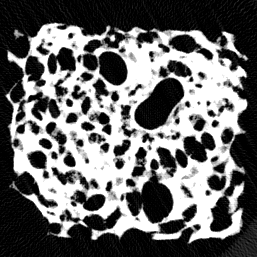
\includegraphics[width=3in]{../figure/answer_3.png}
  \caption{Randon 逆变换还原结果图}
  \label{fig:answer_3}
\end{figure}

解得图 \ref{fig:problem_3} 提供的十个位置处的吸收率如表 \ref{problem_3} 所示。

\begin{table}[htbp]
\centering
\caption{十个位置处的吸收率}
\label{problem_3}
\begin{tabular}{ccccc}
\hline
-0.0175 & 1.4174 & 0.1822 & 0.9373 & 2.0276  \\
\hline
1.8188 & -0.0433 & 0.8058 & 2.9989 & 0.0250  \\
\hline
\end{tabular}
\end{table}

\subsection{问题四}
\subsubsection{问题四的分析}

本题为优化问题,我们在此共采取了两种优化方案:遗传算法优化法和梯度下降优化法,这两种方法都可对系统的精度和稳定性进行分析,也可在一定程度上有所改善。且在本题中,为了方便计算,我们默认CT系统是均匀旋转的。

\subsubsection{两种优化模型的建立及求解}

\textbf{方案一:遗传算法优化法}

我们采用对于重建后图像的每个像素,计算其重建后计算的吸收率 $f(x, y)$ 与题目中所给模型的实际吸收率 $H$ 的差的平方 $E = \frac{1}{2}(f(x, y) - H)^2$ 来衡量重建后的误差,作为损失函数(loss function)。作为最速梯度下降之外的另一方案,我们引入遗传算法(Genetic Algorithm, GA)来对损失函数进行优化。

为了简化计算量与直观表现优化过程与结果,我们设计了新的标定模板,采用一个半径为 $r''$,相对于坐标系原点(附件 1 的图形的椭圆中心)坐标为 $(x'', y'')$ 的圆作为标定方案。保持探测器等间距不变、模型均匀,衰减系数不变(0.77245),重新标定起始角度 $\theta$,每次旋转之后 X 射线顺时针旋转 1 度,依据上文,使用 MATLAB 自身提供的 Radon 与逆 Radon 变换方案进行适合度函数(fitness function)
$$fit(x, y, \theta, r) = \sum_{i = 1}^{256}\sum_{j = 1}^{256}\frac{1}{2}(f(x, y, r, \theta) - H)^2$$
的计算与评估。

设定种群规模为 100,每一代中保持 6 个个体不变,变异概率为 10\%,最小目标值为 3.78,且初代个体在约束区域内随机产生。定义染色体交叉过程
$$mother_1 = k_1 * population(mother), mother_2 = k_2 * population(mother)$$
为母亲一方染色体分裂部分,
$$father_1 = k_1 * population(father), father_2 = k_2 * population(father)$$
为父亲一方染色体分裂部分,$(mother_1, father_2)$,$(mother_2, father_1)$ 分别为两个新个体。相应地,每个个体内基因有 10\% 的概率变异。

最终我们在圆心 (49.84, 36.2), 起始角度 1.224 度,圆半径 3.965mm 取得局部最优解。

\textbf{方案二:梯度下降优化法}

我们在此对问题二中的连续型函数进行误差分析:
$$ E=\iint [f(x,y)-f_1(x,y)]^2\mathrm{d}x\mathrm{d}y $$
令 $ E'=f(x,y)-f_1(x,y) $ ,则由二重数值积分余项公式 
$$ R(f)=-\frac{(d-c)(b-a)}{12}[h_x^2\frac{\partial^2}{\partial x^2}f(\xi_1,\eta_1)+h_y^2\frac{\partial^2}{\partial y^2}f(\xi_2,\eta_2)] $$
可得
\begin{align*}
E' &= \frac{179\theta_0\times511d}{12}[(511d)^2\frac{\partial^2g(\xi_1,\eta_1)}{\partial x^2}+(179\theta_0)^2\frac{\partial^2g(\xi_2,\eta_2)}{\partial y^2}] \\
   &= k_1d^3\theta_0+k_2d\theta_0^3 
\end{align*}

经过化简,可以得到:
$$
\begin{cases}
  k_1=\dfrac{-179\times511^3}{12\pi^2}\dfrac{\cos^2\theta_1}{(x\cos\theta_1-y\sin\theta_1-s_1)^3}\dfrac{\partial p(s_1,\theta_1)}{\partial s}  \\
  k_2=\dfrac{-179^3\times511}{12\pi^2}\dfrac{\sin^2\theta_1}{(x\cos\theta_2-y\sin\theta_2-s_2)^3}\dfrac{\partial p(s_2,\theta_2)}{\partial s}  \\
\end{cases}
$$

此时, $E$ 是关于 $d$ 和 $\theta_0$ 的函数,我们需找到其下降最快的方向。我们设最速下降方向为 $p^k$ ,其表达式为
$$ p^k=-\nabla E(d^k\theta_0^k) $$
设最优步长为 $\lambda_k$ ,且满足
\begin{equation}
\label{equ:E}
E(d^k+\lambda_k\dfrac{<\vec{i},\vec{p^k}>}{\vec{|p^k|}},\theta_0^k+\lambda_k\dfrac{<\vec{j},\vec{p^k}>}{\vec{|p^k|}})
  =\mathop{\min}\limits_\lambda E(d^k+\lambda\dfrac{<\vec{i},\vec{p^k}>}{\vec{|p^k|}},\theta_0^k+\lambda\dfrac{<\vec{j},\vec{p^k}>}{\vec{|p^k|}})
\end{equation} 

在此,我们以已有数据作为初始值开始计算,直至 $\|p^k\|\le\varepsilon$ 时停止,此 $x^k$ 即为所求极值点;否则求最优步长,使得式 \ref{equ:E} 成立,具体流程图如图 \ref{fig:flow} 。

\begin{figure}[htbp]
  \centering
  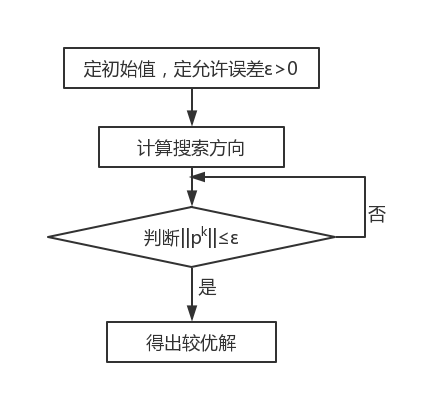
\includegraphics[width=3in]{../figure/flow.png}
  \caption{梯度下降法流程图}
  \label{fig:flow}
\end{figure}

在流程图结束后即可取到理论上 CT 参数的最优解。

% \section{误差分析与灵敏度分析}
% \subsection{误差分析}


% \subsection{灵敏度分析}

\section{模型检验}
问题二、三、四的逆 Radon 变换模型在问题四的优化过程中,同时通过计算误差函数,检验了重建模型的可靠性。总体而言,Radon 变换模型的准确度较高,且仍然有待提升。

\section{模型评价与推广}
\subsection{模型评价}
\subsubsection{模型的优点}
在问题一中,我们通过对附件 2 数据特殊点的位置观测,以及指定某条射线的三次旋转位置关系、圆的相对位置等两种方案确定了附件 1 中均匀介质的吸收率、探测器间距与 180 次的旋转角度,较好的测算了与整个 CT 系统相关的标定参数。

对于问题二、三,我们通过 Radon 变换及其反投影重建逆过程建立了附件 3、附件 5 所示数据的原图像,并通过滤波等图像处理之常见方案对图像进行优化处理,使之更加贴近原像数据,且噪声点得到了较好的处理。

在问题四中,我们提出了最速梯度下降与遗传算法等两种优化吸收率测量误差的方案,并且根据实际情况,建立了遗传算法有关的直观模型,并且实际运算与应用,获得了局部内的最优解。

\subsubsection{模型的缺点}
问题一在最初部分的求解过程依赖于对于特殊位置数据的直接观察,是导致模型不准确的一个潜在因素。

问题二、三的求解过程中,采用的曲面插值方案为线性方案,并以小距离差商代替对应点导数,对应之后二重数值积分求解过程的复化梯形积分。相比于样条方案,线性方案、差商方案难以表现出曲面插值的平滑性,对非观测点的插值结果会产生一定影响。

在问题四的遗传算法求解中,由于运算时间与资源受限,我们仅尝试了小规模的种群数据,根据此数据取得的解仍然有可优化的空间。

\subsection{模型推广}

\bibliography{../reference/bib}

\clearpage
\appendix
\appendixname
\section{程序源码}
以下所有的程序代码均已经包含在支撑材料中,可以通过 MATLAB R2016a 打开支撑材料 /code 文件夹内的 m 扩展名文件来查看。

\begin{lstlisting}[language=MATLAB]
% Question 1

syms r x;
[r, x] = vpasolve([sqrt(r^2 - 1.5257^2) + sqrt(r^2 - 6.2336^2) == 21*x, ...
sqrt(r^2 - 1.5257^2) + sqrt(r^2 - 1.9678^2) == 28*x]);
radiate_weight = abs(r) / 4;
avg_dist = x / radiate_weight;
disp(avg_dist);

attachment_2 = csvread('../resource/attachment-2.csv');
last_k = 0;
result_k = zeros(1,180);

for i = 91:180
%     disp(i);
    end_index = 512;
    for j = 512:-1:1
        if attachment_2(j, i) ~= 0
            end_index = j;
            break;
        end
    end
%     disp(start_index);
    
    calculation_array = attachment_2((end_index - 10):(end_index - 3), i);
%     disp([calculation_array(1), calculation_array(end)]);
    syms k m n;
    a = 15; b = 40;
    [k, m, n] = vpasolve([(sqrt(1+k.^2)/(1 + a.^2*k.^2/b.^2))* ...
    sqrt(4*a.^4*m.^2*k.^2/b.^4 - 4*a^2*(1 + a.^2*k.^2/b.^2) ...
    *(m.^2/b.^2 - 1)) == calculation_array(1)/radiate_weight, ...
        (sqrt(1+k.^2)/(1 + a.^2*k.^2/b.^2))* ...
        sqrt(4*a.^4*n.^2*k.^2/b.^4 - 4*a.^2*(1 + a.^2*k.^2/b.^2)*(n.^2/b.^2 - 1)) ...
         == calculation_array(end)/radiate_weight, ...
        abs(m - n)/sqrt(1 + k.^2) == 7*avg_dist], [k m n]);
    k = abs(k);
%     m = abs(m);
%     n = abs(n);
    if i == 1
        last_k = abs(k);
%         result_k(i) = k;
%         disp(i);
%         disp(k);
        %
        if (atan(k) < 0)
            disp(vpa(2*pi + atan(k)));
        else
            disp(vpa(pi + atan(k)));
        end
        continue;
    else
        if last_k > abs(k)
            k = -abs(k);
            last_k = abs(k);
%             result_k(i) = k;
        else
            last_k = abs(k);
%             result_k(i) = k;
        end
    end
%     disp(i);
%     disp(k);
    if (atan(k) < 0)
        disp(vpa(2*pi + atan(k)));
    else
        disp(vpa(pi + atan(k)));
    end
end

% Question 2

result_shape = zeros(256, 256);
data = csvread('../resource/attachment-3.csv');
data2 = csvread('../resource/attachment-2.csv');
data5 = csvread('../resource/attachment-5.csv');
angles = csvread('../resource/angle_data.csv');
bias_from_1 = 58.8482;
center_x = -6.0874;
center_y = 4.1505;
d = 0.2767;
detector_total_length = 141.6704;
question_data = csvread('../resource/attachment-4.csv');
positions = zeros(10, 2);
result_2 = zeros(10);
result_3 = zeros(10);

% deal with attachment 4
[l, r] = size(question_data);
for i = 1:l
    positions(i, 1) = floor(question_data(i, 1) / (100/256));
    positions(i, 2) = 256 - floor(question_data(i, 2) / (100/256));
%     disp([positions(i, 1), positions(i, 2)]);
end

I1 = iradon(data, rad2deg(angles) - 90, 'linear', 'Ram-Lak', 512);
I2 = imresize(I1, 1/sqrt(2));
disp(length(I2));
[R, C] = size(I2);
I3 = zeros(R, C);
delx = -15; % distance in pixels
dely = -22; % distance in pixels
tras = [1 0 delx; 0 1 dely; 0 0 1];

for i = 1:R
    for j = 1:C
        tmp = [i; j; 1];
        tmp = tras * tmp;
        x = tmp(1,1);
        y = tmp(2,1);
        if (x <= R) && (y <= C) && (x >= 1) && (y >= 1)
            I3(x, y) = I2(i, j);
        end
    end
end;

% imshow(I3);
start_index = floor(length(I3)/2 - 128);
disp(start_index);
I4 = I3(start_index:(start_index + 256), start_index:(start_index + 256));
% imshow(I4);

for i = 1:10
    disp(I4(positions(i, 1), positions(i, 2)));
end

csvwrite('../resource/problem2.csv', I4(1:256, 1:256));

%%%%%%%%%%

I1 = iradon(data5, rad2deg(angles) - 90, 'linear', 'Ram-Lak', 512);
I2 = imresize(I1, 1/sqrt(2));
disp(length(I2));
[R, C] = size(I2);
I3 = zeros(R, C);
delx = -15; % distance in pixels
dely = -22; % distance in pixels
tras = [1 0 delx; 0 1 dely; 0 0 1];

for i = 1:R
    for j = 1:C
        tmp = [i; j; 1];
        tmp = tras * tmp;
        x = tmp(1,1);
        y = tmp(2,1);
        if (x <= R) && (y <= C) && (x >= 1) && (y >= 1)
            I3(x, y) = I2(i, j);
        end
    end
end;

% imshow(I3);
start_index = floor(length(I3)/2 - 128);
disp(start_index);
I4 = I3(start_index:(start_index + 256), start_index:(start_index + 256));
% imshow(I4);

for i = 1:10
    disp(I4(positions(i, 1), positions(i, 2)));
end

csvwrite('../resource/problem3.csv', I4(1:256, 1:256));

% Question 4
% Genetic Algorithm

function [best_fitness, elite, generation] = my_ga(number_of_variables, fitness_function, population_size, parent_number, mutation_rate, maximal_generation, minimal_cost)
    cumulative_probabilities = cumsum((parent_number:-1:1) / sum(parent_number:-1:1));
    best_fitness = ones(maximal_generation, 1);
    elite = zeros(maximal_generation, number_of_variables);
    child_number = population_size - parent_number;
    population = rand(population_size, number_of_variables);

    for generation = 1 : maximal_generation
        cost = feval(fitness_function, population);
        cost = cost(:, 1);
%         disp(cost);
        [cost, index] = sort(cost);
        population = population(index(1:parent_number), :);
        best_fitness(generation) = cost(1);
        elite(generation, :) = population(1, :);
        if best_fitness(generation) < minimal_cost; break; end

        for child = 1:2:child_number
            mother = find(cumulative_probabilities > rand, 1 );
            father = find(cumulative_probabilities > rand, 1 );
            crossover_point = ceil(rand*number_of_variables);
            mask1 = [ones(1, crossover_point), ...
             zeros(1, number_of_variables - crossover_point)];
            mask2 = not(mask1);
            mother_1 = mask1 .* population(mother, :);
            mother_2 = mask2 .* population(mother, :);
            father_1 = mask1 .* population(father, :);
            father_2 = mask2 .* population(father, :);
            population(parent_number + child, :) = mother_1 + father_2;
            population(parent_number+child+1, :) = mother_2 + father_1;
        end

        mutation_population = population(2:population_size, :);
        number_of_elements = (population_size - 1) * number_of_variables;
        number_of_mutations = ceil(number_of_elements * mutation_rate);
        mutation_points = ceil(number_of_elements * rand(1, number_of_mutations));
        mutation_population(mutation_points) = rand(1, number_of_mutations);
        population(2:population_size, :) = mutation_population;
    end
end

% Question 4
% Genetic Algorithm
% Fitness function

function [res] = fitness_function(data)
    center_x = -6.0874;
    center_y = 4.1505;
    w = size(data);
    res = zeros(w(1));
    pixels = zeros(256, 256);
    for index = 1:w(1)
        x = data(index, 1) * 100 - 50;
        y = data(index, 2) * 100 - 50;
        theta_start = data(index, 3) * 360 - 180;
        r = data(index, 4) * 50;
        
        % generate 256 pixels
        x = x - center_x;
        y = y - center_y;
        for i = 1:256
            for j = 1:256
                actual_y = (100/256) * i - 50;
                actual_x = 50 - (100/256) * j;
                if ((actual_x - x)^2 + (actual_y - y)^2) < r^2
                    pixels(i, j) = 1.77245;
                else
                    pixels(i, j) = 0;
                end
            end
        end
        R = radon(pixels, theta_start:(theta_start + 179));
        I = iradon(R, theta_start:(theta_start + 179));
        I = I(1:256, 1:256);
        loss = 0;
        for i = 1:256
            for j = 1:256
                loss = loss + (1/2) * (pixels(i, j) - I(i, j))^2;
            end
        end
       
        res(index) = loss;
    end
end

% Question 4
% Genetic Algorithm

[best_fitness, elite, generation] = ...
 my_ga(4, 'fitness_function', 100, 6, 0.1, 10000, 3.78);
disp(best_fitness(1, :));
disp(elite(1, :));
disp(generation(1, :));

\end{lstlisting}

\end{document}